% fig05_funnel.tex — F-funnel (a)x(b) composite bar chart for the five design points.
% Compiled by the paper Makefile via `make figures` (pdflatex on the snippet).
%
% Data: Table "tab:funnel-rank" of the body, the F-funnel composite ranking.
% Composite = (a) reactivity coverage x (b) Lawson-margin coverage:
%   ITER-class  T=20            -> 0.4843
%   compact-HTS T=20            -> 0.4843
%   ITER-class  T=15            -> 0.3065
%   compact-HTS T=15 (lean tau) -> 0.2939
%   ITER-class  T=10            -> 0.1263
% Verify atoms: f_reactivity_coverage / f_margin_coverage / f_funnel_composite
% (all SUPPORTED-NUMERICAL, |Delta|=0, PR #1020).
%
% Manual single-shot compile (debug):
%   pdflatex -interaction=nonstopmode -halt-on-error fig05_funnel.tex
\documentclass[border=4pt]{standalone}
\usepackage{tikz}
\usepackage{pgfplots}
\pgfplotsset{compat=1.18}
\begin{document}
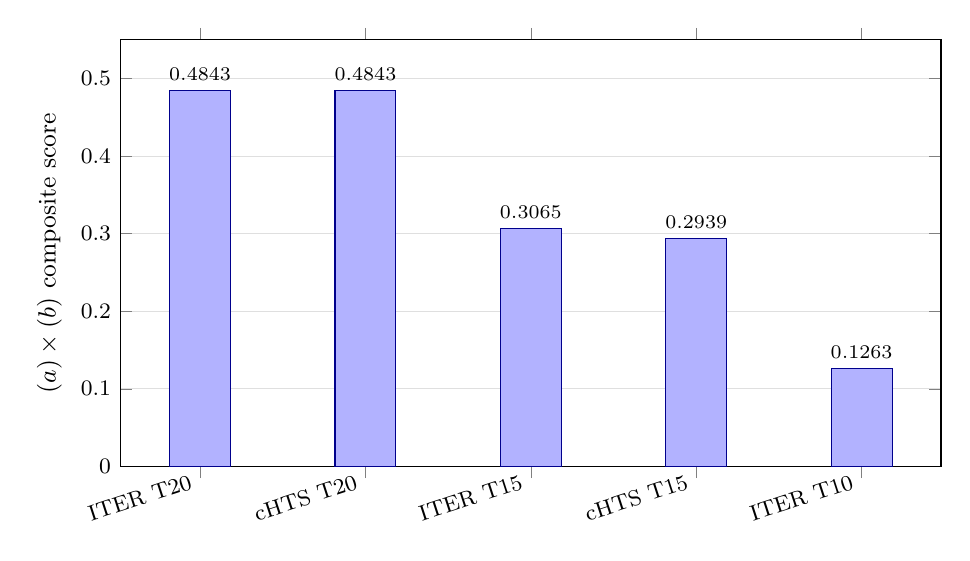
\begin{tikzpicture}
\begin{axis}[
  width=12cm, height=7cm,
  ybar,
  bar width=22pt,
  ymin=0, ymax=0.55,
  ylabel={$(a)\times(b)$ composite score},
  symbolic x coords={ITER T20, cHTS T20, ITER T15, cHTS T15, ITER T10},
  xtick=data,
  x tick label style={font=\footnotesize,rotate=18,anchor=east},
  tick label style={font=\footnotesize},
  label style={font=\small},
  nodes near coords,
  nodes near coords style={font=\scriptsize},
  every node near coord/.append style={/pgf/number format/fixed,
    /pgf/number format/precision=4},
  ymajorgrids,
  grid style={gray!25},
  enlarge x limits=0.12,
]
\addplot[draw=blue!55!black,fill=blue!30] coordinates {
  (ITER T20,0.4843) (cHTS T20,0.4843) (ITER T15,0.3065)
  (cHTS T15,0.2939) (ITER T10,0.1263)
};
\end{axis}
\end{tikzpicture}
\end{document}
